In this section we work through the entire commitment example that has seen used throughout this paper, and we show composition by realizing a coin flipping ideal functionality \Fflip and a protocol realizing it in the \Fcom-hybrid world.
We present the random oracle functionality \Fro, the real world protocol \prot{com}, and a simulator for the dummy adversary.
Along the way we address the apparent import mismatch between \Fcom and \Fro, and we discuss how emulation and composition work around it.
Finally, we give \Fflip, and a realizing protocol and sketch the composed simulator for $\Fro \xrightarrow{\prot{flip} \circ \prot{com}} \Fflip$.

\subsection{The Random Oracle}
The random oracle functionality captures an idealized hash function. It samples random strings of length $k$ as ``hash values`` and stores them in a table for deterministic hashes.
It allows both protocol parties and the adversary to send 1 import token and request hashes from it
We augment \Fro with a single communication channel allowing it parties to send messages to each other. One caveat from traditional communication
is that the protocol parties must poll \Fro for new messages. The augmented functionality is called \Fropp from now on.

The random oracle is different from \Fcom in that it has one channel to all parties to use. This is due to the fact that its function is the same for all parties.
Recall the session type and its structure discussed in Section~\ref{sec:execuc}. The augmented session type is given below:
%The design of the random oracle is different from \Fcom in that it has only one channel for all parties to communicate over.
%We discussed the unique structure of the session type for \Fro in Section~\ref{sec:execuc}: its type before and after interaction with a party is the same.
%This enables a dynamic set of parties to communicate with it by moving the \inline{pid} of the message sender/receiver into the type.
%Our augmented functionality's type retains this feature, as described by its session type:
%\begin{mathpar}
\begin{center}
\parbox{0cm}{
\begin{tabbing}
$\m{party}[a] = \textcolor{red}{\getpot^2} \ichoice{$\=$\mb{hash}: \m{pid} \arrow \m{int} \tensor \echoice{$\=$\mb{shash}: \m{pid} \arrow \m{int} \tensor \textcolor{red}{\paypot^1} \m{party[a]}}$ \\
\>$\mb{recv}: \m{pid} \tensor \echoice{$\=$\mb{yes}: \m{pid} \arrow \m{pid} \arrow \m{a} \tensor \textcolor{red}{\paypot^1} \m{party}[a],$\\
\>\>$\mb{no}: \m{pid} \tensor \m{party[a]}},$ \\
\>$\mb{send}: \m{pid} \arrow \m{pid} \arrow \m{a} \tensor \m{party}[a]}$
%$\m{party}[a] = \textcolor{red}{\getpot^2} \ichoice{$\=$\mb{hash} : \m{pid} \arrow \m{int} \tensor \m{hashing}[a],$\\
%\>$\mb{send} : \m{pid} \arrow \m{pid} \arrow \m{a} \tensor \m{party}[a],$ \\
%\>$\mb{recv}: \m{pid} \tensor \m{newmsg[a]}}$ \\
%$\m{hashing}[a] = \echoice{\mb{shash} : \m{pid} \arrow \m{int} \tensor \textcolor{red}{\paypot^1} \m{party}[a]}$ \\
%$\m{newmsg}[a] = \echoice{ \mb{yes}: \m{pid} \arrow \m{pid} \arrow \m{a} \tensor \textcolor{red}{\paypot^1} \m{party}[a], \mb{no}: \m{pid} \tensor \m{party[a]}}$
%\end{mathpar}
\end{tabbing}}
\end{center}
Similarly, the functional types are given by:
%One side effect of the session types is that we modify the standard UC channel to require receivers to ask for new messages sent to them.
%We cannot directly deliver messages to their receivers, because the committer's and receiver's \inline{p2f} channel would end up with different types and back to \inline{party[a]}.
%The corresponding functional message type between the protocol wrapper and functionality is also updated with inputs for the channel:
\begin{lstlisting}[basicstyle=\footnotesize\BeraMonottFamily, mathescape]
$\Type$ rop2f[a] = QHash of $\tgr{Int}$ | Send of pid ^ a 
               | Recv ;
$\Type$ rof2p[a] = RHash of $\tgr{Int}$ | Yes of pid ^ a 
               | No ;
\end{lstlisting}

\subsection{Commitment Protocol}
The real world commitment protocol is constructed in the random oracle model in the way of ~\cite{hofheinzcommitment}.
Its incoming channel from \Z is typed identically to \Fcom to ensure that emulation and composition hold.

We show a snippet of the sender code for computing the commitment for its input bit in Figure~\ref{lst:committer}, and the relevant code the the receiver checking the commitment in Figure~\ref{lst:receiver}.
The sender accepts a bit from its \inline{z2p} channel and generates a nonce to blind the bit through a \inline{sample} of randomness~\footnote{Blinding is necessary otherwise \A knows the pre-image and can query \Fro for its hash value.}.
It creates the commitment by sending \Fropp the blinded bit and receiving a hash value from \inline{p2f}.
Finally it sends the hash to the receiver (which has pid=2).
Conversely, the receiver must request the commitment \inline{h} message from \Fropp, notify \Z of the commitment, and, as shown in Figure~\ref{lst:receiver}, when it receives the bit and the nonce it checks that its hash with the commitment.
%$\tb{case}$ $\$$z2p (
%  commit => 
\begin{figure}
\begin{lstlisting}[basicstyle=\footnotesize\BeraMonottFamily, frame=single, mathescape]
$\tg{(* committer code after receiving a 'commit' message from the environment *)}$
b = $\tm{recv}$ $\$$z2p ;
$\nget$ $\$$z2p {1} ;
bits = sample k rng ;
$\$$p2f.hash ;
$\npay$ $\$$p2f {2} ;
$\tm{send}$ $\$$p2f pid ;
$\tm{send}$ $\$$p2f b + bits ;
$\tb{case}$ $\$$p2f (
  shash => 
    h = $\tm{recv}$ $\$$p2f ;
    $\$$p2f.send ;
    $\tm{send}$ $\$$p2f pid 2 hash;
\end{lstlisting}
\caption{The code for the committer in $\prot{com}$ when it receives a \msf{commit} message from \Z. It obtains a hash of the message from \Fropp over \msf{p2f} and sends it to the receiver (pid=2) through the same functionality.}
\label{lst:committer}
\vspace{-2mm}
\end{figure}
%$\$$p2f.recvmsg ;
%$\tb{case}$ $\$$p2f (
%  Yes(p, h)
%  $\tm{recv}$ $\$$p2f ;
%...
%$\tm{send}$ $\$$p2f (b+h);
%...
\begin{figure}
\begin{lstlisting}[basicstyle=\footnotesize\BeraMonottFamily, frame=single, mathescape]
$\tg{(* receiver waiting for the commitment opening from the random oracle channel *)}$
sender = $\tm{recv}$ $\$$f2p ;
(b,h) = recv $\tm{recv}$ $\$$f2p ;
$\nget$ $\$$f2p {1} ; 
$\tg{(* query the hash of b+h with 1 import *)}$
h = $\tm{recv}$ $\$$p2f ;
$\yo{if}$ h == hash
$\yo{then}$
  $\$$z2p.open
$\yo{end}$
\end{lstlisting}
\caption{The code for the receiver checks for a new message and receives the bit and nonce from the committer. If the hash of the bit and nonce matches the commitment it received, it returns \msf{open} to \Z to confirm the commitment.}
\label{lst:receiver}
\vspace{-3mm}
\end{figure}

%The protocol works as follows:
%\begin{enumerate}
%\item When the committer receives a \inline{Commit(b)} message from \Z, it samples some random bits $r$ and generates a hash $h$ by sending \inline{SHash(b + r)} to \Fro.
%\item It then sends the commitment to the receiver who notifies \Z with a \inline{committed} message.
%\item Finally, when \Z instructs the committer to \inline{Open} the commitment, it sends bit \inline{b} and randomness \inline{r} to the receiver. The receiver checks the commitment, with \inline{b} and \inline{r}, against \Fro and outputs \inline{Open(b)} to \Z if it checks out.
%\end{enumerate}

\subsection{Simulation}
Finally, we present a simulator \simcom, for the dummy adversary, for which the \Fcom is realized by \prot{com} in the \Fropp-hybrid world.
Recall that the import requirements for the ideal world, in this case for \Fcom. Therefore, the simulator is parameterized by import parameters required in the real world for the parties of $\pi_\m{com}$ and \Fro.
The simulator is straightforward and internally maintains a table like \Fro and responds to the environments queries for hashes. 
When the receiver is corrupt:
\begin{itemize}
\item \simcom responds with \inline{P2A2Z(2, no)} to all messages by \Z to get a message from the functionality
\item On \inline{Committed} by the ideal receiver, \simcom generates a random $r$ and sends \inline{P2A2Z(2, RHash(h))} with no import.
\item On \inline{Open(b)} from the ideal receiver, \simcom generates a random nonce $x$ and stores \inline{b+x : h} in its \Fro table, and sends \inline{Yes(1, (b,x))} to \Z when asked for messages for the corrupt receiver.
\end{itemize}

The corrupt committer is not much different from the above case. In this case
the simulator stores the bit $b$, the none $x$, the corresponding hash $h$, and the import that \Z uses to create a commitment.
When the simulator receives the message to send the commitment to the receiver, it tells the ideal world committer to commit to $b$ along with 2 import given by \Z, and when it's told to open the commitment it opens it in the ideal world. 

It is immediately clear that this simulator satisfied $\Fro \xrightarrow{\prot{com}} \Fcom$ for the dummy adversary.

\subsection{Coin Flipping}
We present secure coin flipping here as another example and one that makes use of our composition operator. 
Additionally, this example makes use of a neat trick we use to get more guarantees out of the NomosUC type system.
Securely flipping a coin is a basic cryptographic primitive whose ideal functilnalitt \Fflip is captured by the session types in Figure~\ref{fig:fflip}.
It's a 2-party protocol where one party is the initiator of the flip and the other is a receiver.
The desired property is that the coin flip is entirely unbiased by either of the two parties. The corresponding ideal functionality \Fflip samples a bit from from its random tape and returns it as the coin flip.
\begin{figure}
\begin{center}
\parbox{0cm}{
\begin{tabbing}
	$\m{flip[K]\{n\}\{m\}} = \textcolor{red}{\getpot^n} \; \ichoice{\mb{init}: K \arrow \ichoice{\mb{getflip}:  \echoice{ $\=$\textcolor{red}{\getpot^m}\mb{yes}: Bit \product 1,$ \\
	\>$\textcolor{red}{\getpot^m} \mb{no}: \m{flipped}[K]}}}$ \\
	$\m{receiver[K]\{n\}\{m\}} = \textcolor{red}{\paypot^n} \ichoice{\mb{getflip}: \echoice{$\=$ \textcolor{red}{\getpot^m}\mb{yes}: Bit \product 1,$\\
	\>$\textcolor{red}{\paypot^m} \mb{no}: \m{receiver[K]}}}$ \\
	$\m{adv[K]\{n\}} = \textcolor{red}{\getpot^n}\echoice{\mb{flip}: K \arrow \echoice{\mb{flipok}: \ichoice{$\=$\mb{yes}: 1,$\\
	\>$\mb{no}: 1}}}$
\end{tabbing}}
\end{center}
\caption{The session types describing \Fflip's channels with the flipper, receiver, and the adversary.}
\label{fig:fliptype}
\vspace{-4mm}
\end{figure}

%\begin{figure}
%\centering
%\begin{lstlisting}[basicstyle=\footnotesize\BeraMonottFamily, frame=single, mathescape]
%$\Type$ flipper[K] = +{ init: K -> flipped } ;
%$\Type$ fflipped = +{ getflip: &{ flip: Bit * 1 ,
%                                  noflip: fflipped }} ;
%$\Type$ receiver[K] = +{ getflip: &{ flip: K -> Bit -> 1 ,
%                                     noflip: recever[K] }} ;
%$\Type$ adv[K] = &{ flipped: K -> deliver } ;
%$\Type$ deliver = &{ askflip: +{ yes: deliver,
%                                 no: deliver }}
%\end{lstlisting}
%\end{figure}

\Fflip only sends messages to the receiver when asked for the outcome of the flip with a \inline{getflip}. 
We augment the session type, and the corresponding ideal functionality, with a polymorphic \inline{K} to strengthen the type and ensure that the receiver can not receive anything from \inline{getflip} until the flipped sends something of type \inline{K} to \Fflip.
We concretize \inline{K} with the unit type \inline{()} at the protocol level as we only care about ordering in the functionality. 
This gives the type more power and allows the resulting functionality and protocol code to be simpler. 

The code for \Fflip is quite simple and shown below:
\begin{lstlisting}[basicstyle=\footnotesize\BeraMonottFamily, frame=single, mathescape]
$\nproc$ F_coinflip[K]{p2fn}{m} :
  (k: Int), (rng: [Bit]), (sid: session[1]),
  ($\$$F: flipper[$\tp{K}$]{$\tp{p2fn}$}{$\tp{f2pn}$}), ($\$$R: receiver[$\tp{K}$]{$\tp{p2fn}$}{$\tp{f2pn}$}),
  ($\$$A: adv[$\tp{K}$]) |- ($\$$c: 1) =
{
  $\ncase$ $\$$F (
    init =>
      x = $\nrecv$ $\$$F ;
      $\nget$ $\$$F {p2fn}
      b = sample 1 rng ;
      $\$$A.flipped ;
      $\nsend$ $\$$A x ;
      $\tg{(* wait for getflips *)}$
      $\$$f <- getflip_f{$\tp{p2fn}$}{$\tp{f2pn}$} <- b $\$$F ;
      $\$$r <- getflip_r[$\tp{K}$]{$\tp{p2fn}$}{$\tp{f2pn}$} <- b x $\$$R ;
  )
}
\end{lstlisting}
We elide the code for \inline{getflip} although it is straightforward. 
The adversary decides whether to deliver the output flip to a party asking for it.
Much like the real-world case where the corrupt committer never opens its commitment, the simulator here can ensure that only the flipper receives the flip.
As the session type indicates, the adversary responds with a \inline{yes} or \inline{no} to deliver the flip.

%Upon a \inline{getflip} request, the adversary is activated and asked whether to deliver the outcome as shown in Figure~\ref{fig:optional}. 
%\begin{figure}
%\centering
%\begin{lstlisting}[basicstyle=\small\BeraMonottFamily, frame=single, mathescape]
%$\ncase$ $\$$F (
%  getflip =>
%    $\$$A.askflip ;
%    $\ncase$ $\$$A (
%      yes =>
%        $\$$F.flip ; send $\$$F b ;
%      no =>
%        $\tg{(* loop and wait for getflip *)}$
%    )
%)
%\end{lstlisting}
%\caption{} \label{fig:optional}
%\end{figure}

The protocol for the coin flip uses \Fcom. 
The flipper commits to a bit $b$, the receiver sends the flipper a random bit $r$ in return, the flipper opens its commitment, and both parties compute the flip as $r \oplus b$.
The simulator for this protocol to realize \Fflip is straightforward:
\begin{itemize}
\item If the flipper is corrupt, the simulator tells the flipper to \inline{init} the flip when the environment sends it a \inline{Commit b} message. It gets the flip outcome $f$ from the flipper and simulates the receivers random bit $r = f \oplus b$ for the environment. It never delivers the flip outcome to the receiver unless the environment instructs it to open the flipper's commitment. By setting $r = f \oplus b$, when the environment receives $f$ it can check that $r \oplus b = f$.
\item If the receiver is corrupt, the simulator waits for \Fflip to inform it that the flip was initiated. It simulates the \inline{Commit} message from \Fcom to the receiver, for \Z. When it receives the random bit that \Z wants the receiver to send, it gets the flip outcome from the receiver, computes $b = r \oplus f$ and sends \inline{Open b} to \Z. Again, \Z can verify $b \oplus r$ similar to the above case.
nl
\end{itemize}

\subsection{Composition}
We describe a composition theorem in the previous section and a composition operator for protocols.
Here we demonstrate how to compose the simulators from the two experiments to create a simulator to prove Theorem~\ref{thm:compose}.
Two simulators being composed are: \SIM{com} for $\Fro \xrightarrow{\prot{com}} \Fcom$ and \SIM{flip} for $\Fcom \xrightarrow{\prot{flip}} \Fflip$. 
The code for the composed is very similar to the simulator for the Dummy Lemma described in Section~\ref{sec:dummy} and expanded on in Appendix~\ref{app:dummy}.
The exact connects are different but it follows identical virtualization and sandboxing.
Therefore, we elide any code snippets from this section and, instead, present a high-level description of the simulator.

For the sake of generality, we refer to protocols $\pi$, $\rho$, and functionalities $\F_1$, $\F_2$, and $\F_3$, where $\rho$ is \prot{flip}, $\pi$ is \prot{com}, $\F_1$ is \Fro, $\F_2$ is \Fcom, and $\F_3$ is \Fflip.
The numbered steps in the description below correspond to the numbered arrows in Figure~\ref{fig:simcomp}.
\begin{enumerate}
\item Input from \Z: \inline{Z2A2P(p, msg)} for dummy parties of $\F_1$ and \inline{Z2A2F(msg)} for $\F_1$  are forwarded to \SIM{\pi}, and, Outputs from \SIM{\pi}: \inline{F2A2Z(msg)} and \inline{P2A2Z(p,msg)} are forwarded to \Z unaltered.
\item Inputs from \SIM{\pi}: \inline{A2F(msg)} for $\F_2$ and \inline{A2P(msg)} for dummy parties of $\F_2$ are forwarded to \SIM{\rho} as \inline{Z2A2F(msg)} \inline{Z2A2P(p,msg)}, respectively.
\item Outputs from \SIM{\rho}: \inline{P2A2Z(p,msg)} from simulated parties of $\rho$  and \inline{F2A2Z(msg)} from the simulated $\F_2$ are forwarded to \SIM{\pi} as \inline{P2A(p,m)} and \inline{F2A(m)}, respectively.
\item Inputs from \SIM{\rho}: \inline{A2F(msg)} for $\F_3$ and \inline{A2P(p,msg)} for dummy parties of $\F_3$ are forwarded unaltered, and, Outputs from $\F_3$ and its ideal parties: \inline{F2A(msg)} from $\F_3$ and \inline{P2A(p,msg)} from its ideal parties is forwarded to \SIM{\rho} unaltered.
\end{enumerate}

\begin{figure}
\centering
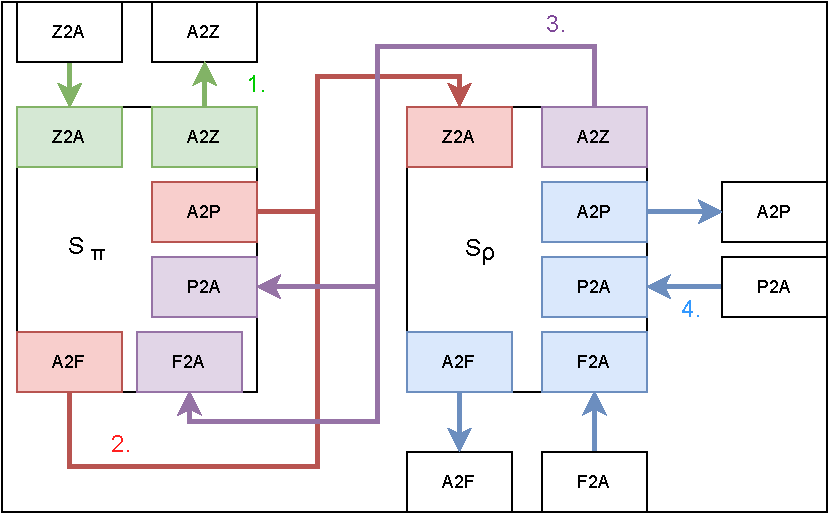
\includegraphics[scale=0.5]{figures/simcomp.pdf}
\caption{The composed simulators for $\F_1 \xrightarrow{\rho \circ \pi} \F_3$. The real world consists of $(\rho \circ \pi, \F_1)$. Inputs from \Z are for $\F_1$ and dummy parties interacting with $\F_1$, which \SIM{\pi} is equipped to handle. Outputs from \SIM{\pi} are for $\F_2$ and dummy parties of $\F_2$ which \SIM{\rho} is equipped to handle. Finally, outputs from \SIM{\rho} are for $\F_3$ and dummy parties of $\F_3$, which is just the ideal world in Theorem~\ref{thm:composition}.}
\label{fig:simcomp}
\end{figure}


The type system in NomosUC helps to identify when the amount of potential that a functionality requires isn't satisfied by the bounding polynomial given.
We illustrate this point using the $\F_{\msf{map}}$. 
The functionality maintains a list that parties can append to the end of or read from.

